
\documentclass[linenumbers,trackchanges]{aastex7}

\newcommand{\vdag}{(v)^\dagger}
\newcommand\aastex{AAS\TeX}
\newcommand\latex{La\TeX}
\usepackage{float}
\usepackage{amsmath}
\begin{document}

\title{CTA200 Assignment 3}


\author[]{Nava Wolfish}
\affiliation{University of Toronto}
\email[show]{nava.wolfish@mail.utoronto.ca}  


\section{Question 1} 
For this question, we were tasked with recreating the Mandelbrot set. This set is defined by all $c = x + iy$, $-2 \leq x \leq 2$, $-2 \leq y \leq 2$, such that the sequence in Equation \ref{eq:mandeleq} converges absolutely for $z_0 = 0$. 
\begin{equation}\label{eq:mandeleq}
     z_{i+1} = z_i^2 + c
\end{equation}

To perform this calculation in python, I first used \verb|numpy.meshgrid| to define $(1000 \times 1000)$ coordinates for $c$ within the desired range.

Next, I created a function (\verb|mandelbrot_iteration|) containing a loop that would repeat the calculation of $z_i$ for a maximum number of iterations \verb|max_iter|. \verb|numpy|'s built-in capabilities allows me to perform the calculation for all $c$ simultaneously. At each iteration, the function checks which $|z|$ have surpassed some \verb|arb_limit|. If $|z|$ has diverged, the function stores the iteration number in a new array (\verb|conv|), mutually indexed to $c$ and $z$. If the sequence doesn't converge, then \verb|conv| stores \verb|max_iter|. 

Once the maximum number of iterations has been reached, my function returns \verb|conv| and the array of $z$ values. 

I stored this function in a separate python script \verb|complex_iteration.py|. In my notebook, I called the function for my array of $c$ values, and the parameters \verb|arb_limit = 1e6|, \verb|max_iter = 50|. First I used \verb|plt.contourf| to visualize the number of iterations required for $z$ to converge for each $c$. This plot is shown in Figure \ref{fig:q1p1}.

\begin{figure}[h!]
\plotone{figures/q1p1.png}
\caption{Visualization of the number of iterations required for $z$ to converge for each $c$. I obtain the Mandelbrot set as visualized in \citet{avalos-bock}.}
\label{fig:q1p1}
\end{figure}

Next, I used \verb|conv| to display the set of convergent $c$. Yet again, I obtain the Mandelbrot set, as visualized in Figure \ref{fig:q1p2}. 

\begin{figure}[h!]
     \plotone{figures/q1p2.png}
     \caption{Visualization of the the Mandelbrot set. The darker magenta represents $c$ such that $z$ converges, while the light pink is the divergent region.}
     \label{fig:q1p2}
\end{figure}
\section{Question 2}
In this question, we were tasked with recreating the integration of the system described in \citet{lorenz_deterministic_1963}. The system is given in Equation \ref{eq:system}, where $\sigma$, $r$, and $b$ are constants. In my analysis, I integrate this system from $t = 0$ to $t = 60$, with a timestep of $dt = 0.01$.
\begin{align}\label{eq:system}
     \dot{X} &= -\sigma (X - Y)\\
     \dot{Y} &= rX - Y - XZ\\
     \dot{Z} &= -bZ + XY\\
\end{align}
First, I create a function in python (\verb|lorenz_system|) that takes in $t, X, Y, Z$ in addition to the parameters $\sigma, r, b$. The function returns a vector $\dot{W} = (\dot{X}, \dot{Y}, \dot{Z})$. I set $\sigma = 10.$, $r = 28$, and $b = 8./3.$ as specified in \citet{lorenz_deterministic_1963}. Next, using the initial guess $W_0 = (0., 1., 0.)$, I used \verb|scipy.optimize.solve_ivp| to develop a solution. In my analysis, I integrate the system from $t = 0$ to $t = 60$, with a timestep of $dt = 0.01$.

Figure \ref{q2p3} contains the solution for $Y$ from $t = 0$ to $t = 30$. This figure is comparable to Lorenz's Fig 1, which displays similar results. My integration, similarly to Lorenz's, displays inconsistent oscillations after $N \approx 1600$. While the shape of these oscillations are the same, the sign differs with Lorenz's results. I attribute these deviations to a difference in integration methods in both analyses.
\begin{figure}[h!]
     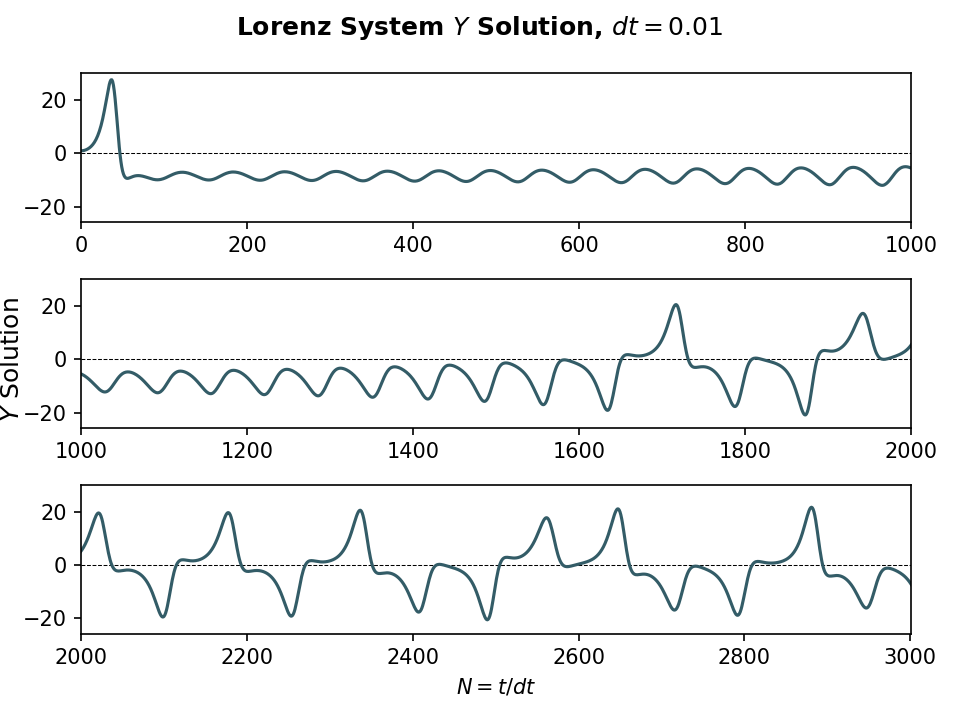
\includegraphics{figures/q3p3.png}
     \caption{my Recreation of Figure 1 in \citet{lorenz_deterministic_1963}. We see a slight deviation from the results from the paper after $N \approx 1600$, attributed to the difference in numerical integration techniques. }
     \label{q2p3}
\end{figure}

I can also plot the phase space of my solutions from $t = 14$ to $t = 19$, as shown in Figures \ref{q3p4a} and \ref{q3p4b}. Again, these are visually similar to Lorenz's Figure 2. The deviations in the results are again attributed to difference in integration methods.
\begin{figure}[h!]
     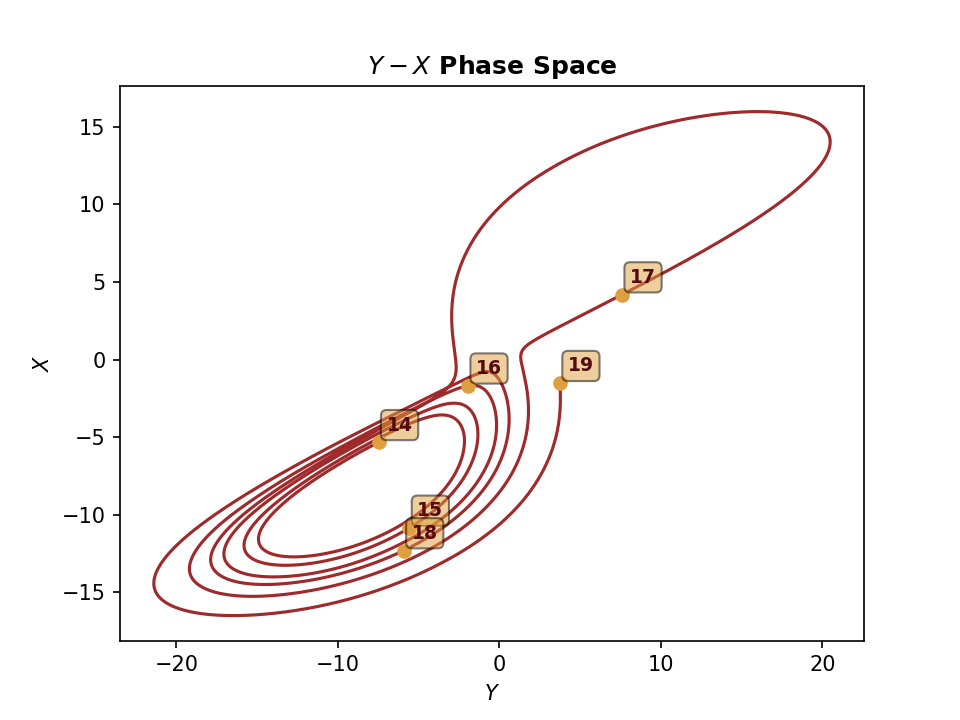
\includegraphics{figures/q3p4a.png}
     \caption{Phase Space of $Y-X$ Solution from $t = 14$ to $tb = 19$.}
     \label{q3p4a}
\end{figure}
\begin{figure}[h!]
     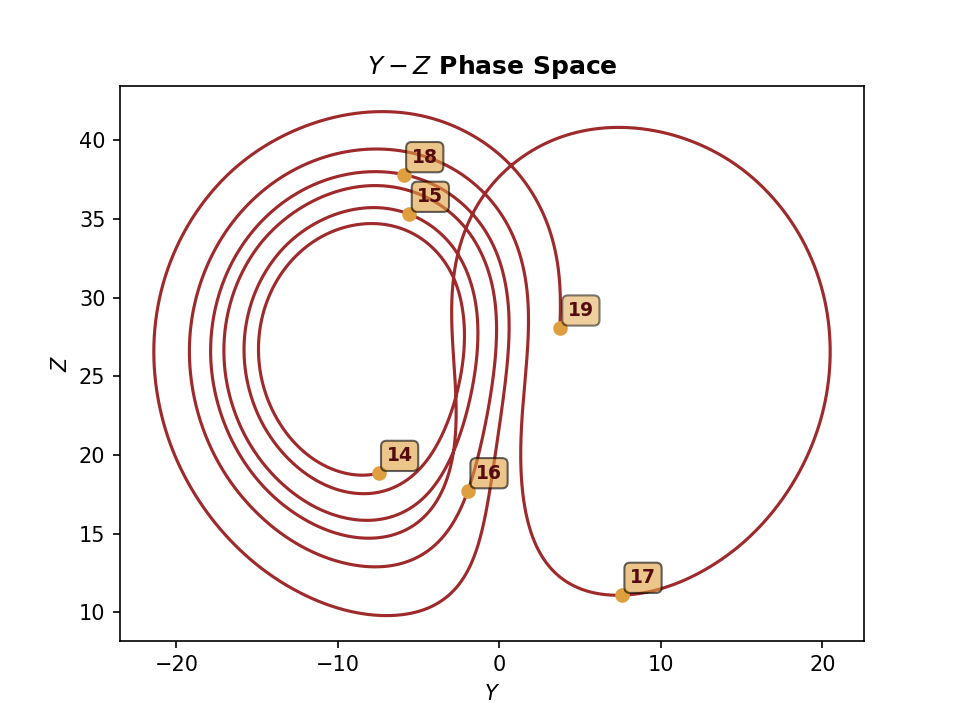
\includegraphics{figures/q3p4b.png}
     \caption{Phase Space of $Y-Y$ Solution from $t = 14$ to $tb = 19$.}
     \label{q3p4b}
\end{figure}

Lastly, I examine the effects of small perturbations on the solution. I reintegrate the system, this time with initial condition $W_0' = (0. 1. + 1e-8, 0.)$. I calculate the distance between the corresponding solution $W'$ and the original solution $W$. A plot of the distance between the two solutions over time is shown in \ref{fig:q5p5}. The result is roughly linear growth in the perturbation over time. The growth of the perturbation indicates that the equilibrium state of the solution is unstable. 

\begin{figure}
     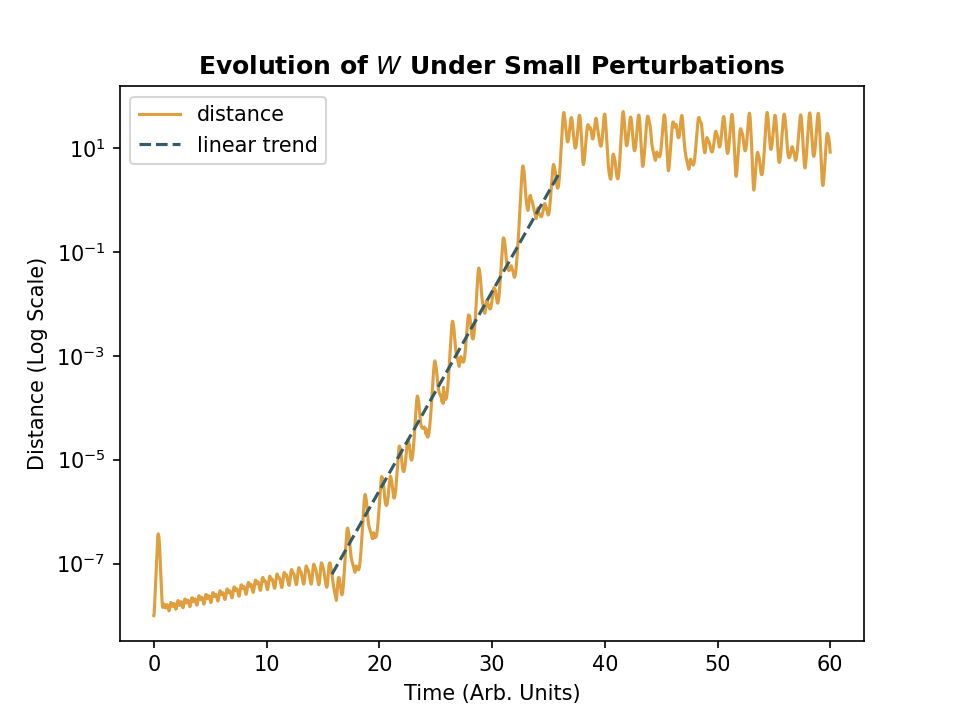
\includegraphics{figures/q3p5.png}
     \caption{Distance between solutions of the system under small perturbations. The roughly linear behaviour indicates that the equilibrium of the system is unstable.}
     \label{fig:q5p5}
\end{figure}
\section{Floats} \label{sec:floats}


%% For this sample we use BibTeX plus aasjournalv7.bst to generate the
%% the bibliography. The sample7.bib file was populated from ADS. To
%% get the citations to show in the compiled file do the following:
%%
%% pdflatex sample7.tex
%% bibtext sample7
%% pdflatex sample7.tex
%% pdflatex sample7.tex

\bibliography{sample7}{}
\bibliographystyle{aasjournalv7}

%% This command is needed to show the entire author+affiliation list when
%% the collaboration and author truncation commands are used.  It has to
%% go at the end of the manuscript.
%\allauthors

%% Include this line if you are using the \added, \replaced, \deleted
%% commands to see a summary list of all changes at the end of the article.
%\listofchanges

\end{document}

% End of file `sample7.tex'.
